%\documentclass[preprint,prl]{revtex4}

\documentclass[prl]{revtex4}

\usepackage{ORI_Group_style}
\usepackage{siunitx}


\graphicspath{{./figs/}}


\begin{document}

\title{Photophysics of Nitrogen Vacancy centres in Nanodiamonds}
  
\author{Reece P. Roberts$^{1,2}$}
\author{Author2$^{1,2}$}

\affiliation{$^1$ Department of Physics \& Astronomy, Macquarie University, NSW 2109, Australia}
\affiliation{$^2$ ARC Centre for Engineered Quantum Systems, Macquarie University, NSW 2109, Australia}


\begin{abstract}
I will write my abstract when I know my exact story.
The paper will be two papers, one for 780nm and one for 1042nm, unless I gain by putting the two papers together and build one higher impact paper.
The complete set of data should answer this question.
For example is there a difference between the mechanisms for each wavelength. For example the 780nm can both ionise and recombine, however maybe the 1042nm can only ionise and can't lease to a recombination process.
\end{abstract}

\maketitle

\section{Introduction}
\subsection{What is it and why is it important?}
The Nitrogen Vacancy (NV) centre is is a point defect consisting of a nitrogen-vacancy lattice pair embedded along the [111] axis of a diamond (???ref1). The NV centre has two stable charge states, the neutral charge state (NV$^0$) and the negatively charged state (NV$^-$), with photo-induced interconversion between these two states (???ref2). The NV$^-$ charge state is an intensively studied material that has shown a wide range of applications in both Physics and Biology due to it's high stability and interesting optical properties. Biologists have used them extensively for biolabelling and imaging of internal biological structures (???ref3). For example the surface of nanodiamonds can be functionalised and internalised by cells without toxic effects and once bonded to the target they can be imaged by using the unique optical properties of the embedded defect(???ref4). Meanwhile, Physisits have been investigating their uses in wide range of nanoscale sensing and quantum sensing applications(???ref5). By exploiting the quantum mechanical interactions of the defects internal spin state the NV$^-$ centre has been used to observe quantum behaviour at room temperature, providing a platform to study a wide variety of quantum manipulation protocols (???ref6). However these effects rely on only the NV$^-$ charge state and often neglect the  existence of the NV$^0$ charge state. 

In many applications only the NV$^-$ charge state is desired and in order to obtain the largest charge state polarisation in the NV$^-$ charge state the excitation photophyics of the NV centre were investigated(ref7???). Excitation wavelengths from 450-610nm were probed and an optimal excitation wavelength was stated to be around 510-540nm, although the charge state polarisation was always $\leq$75\%. For most applications invoving NV centres an excitation wavelength in the region was chosen, typically 532nm, and the effects of the NV$^0$ charge state were ignored.

\subsection{Problem}

The NV has long been stated to be extremely robust, with no bleaching or blinking under normal conditions(ref8???). However, in many cases once a second probe laser is used in an experiment the Fluorescence of the NV centre is dramatically quenched(ref9???) limiting its use in further applications and in conjunction with other systems. The quenching of fluorescence has been observed and described by numerous potential mechanisms, including make list here(???1). In contrast to these many of these mechanisms we are collecting the fluorescence of both charge states as well as probing in a non resonant continuous-wave regime of a few 10s of milliwats eliminating many of the above mechanisms. Interestingly the quenching mechanism at ~780nm has been observed, used and described as a stimulated emission depletion (STED) process for imaging(ref10???). Recently however, in the field it has been noted that this effect is not a true STED process even though it still gives the same desirable effect (ref11???).  

\subsection{How do we fill in gap of knowledge?}

In this paper we investigate the quenching effects of the NV centre fluorescence in order to provide insight into the charge and spin state photo-dynamics. Our process is to measure the quenching dynamics of the NV centre under steady state illumination and using established physics of the NV centre, develop a rate equation model to describe the photo-physics of the system. Using this model various assumptions are analysed to determine their validity and the most likely model that closely represents the photo-physics is determined by the Aikike information criteria. We believe this new rate equation model has now identified the underlying physics leading to the quenching of fluorescence of NV centres and it now allows us to predictively simulate and optimise the effect. By understanding the appropriate rates we can apply particular initialisation processes to increase the spin and charge state polarisation of the NV centre which will lead to direct enhancements of existing applications including applications such as STED like imaging and for enhancing state preparation for NV based quantum technologies.

\section{Experiment}
\subsection{Setup}
In our experiment, (???2) type and size nanodiamonds are dispersed on a glass coverslip placed on the sample plane of a custom built scanning confocal microscope. The NV centres are pumped with a 532nm continuous wave laser after focusing through a x.xNA, Brand, type immersion objective lens ???3. The 780nm and 1042nm lasers are combined and then superimposed with the 532nm laser before the objective lens. The fluorescence is collected through the same objective and sent to an avalanche photodiode. A permanent neodymium magnet was placed on a moveable arm above the sample plane so that a large non zero magnetic field could be brought in close proximity to the nanodiamond. The setup is shown in Fig. \ref{FigSetup}.

\begin{figure}[t]
  \centering
  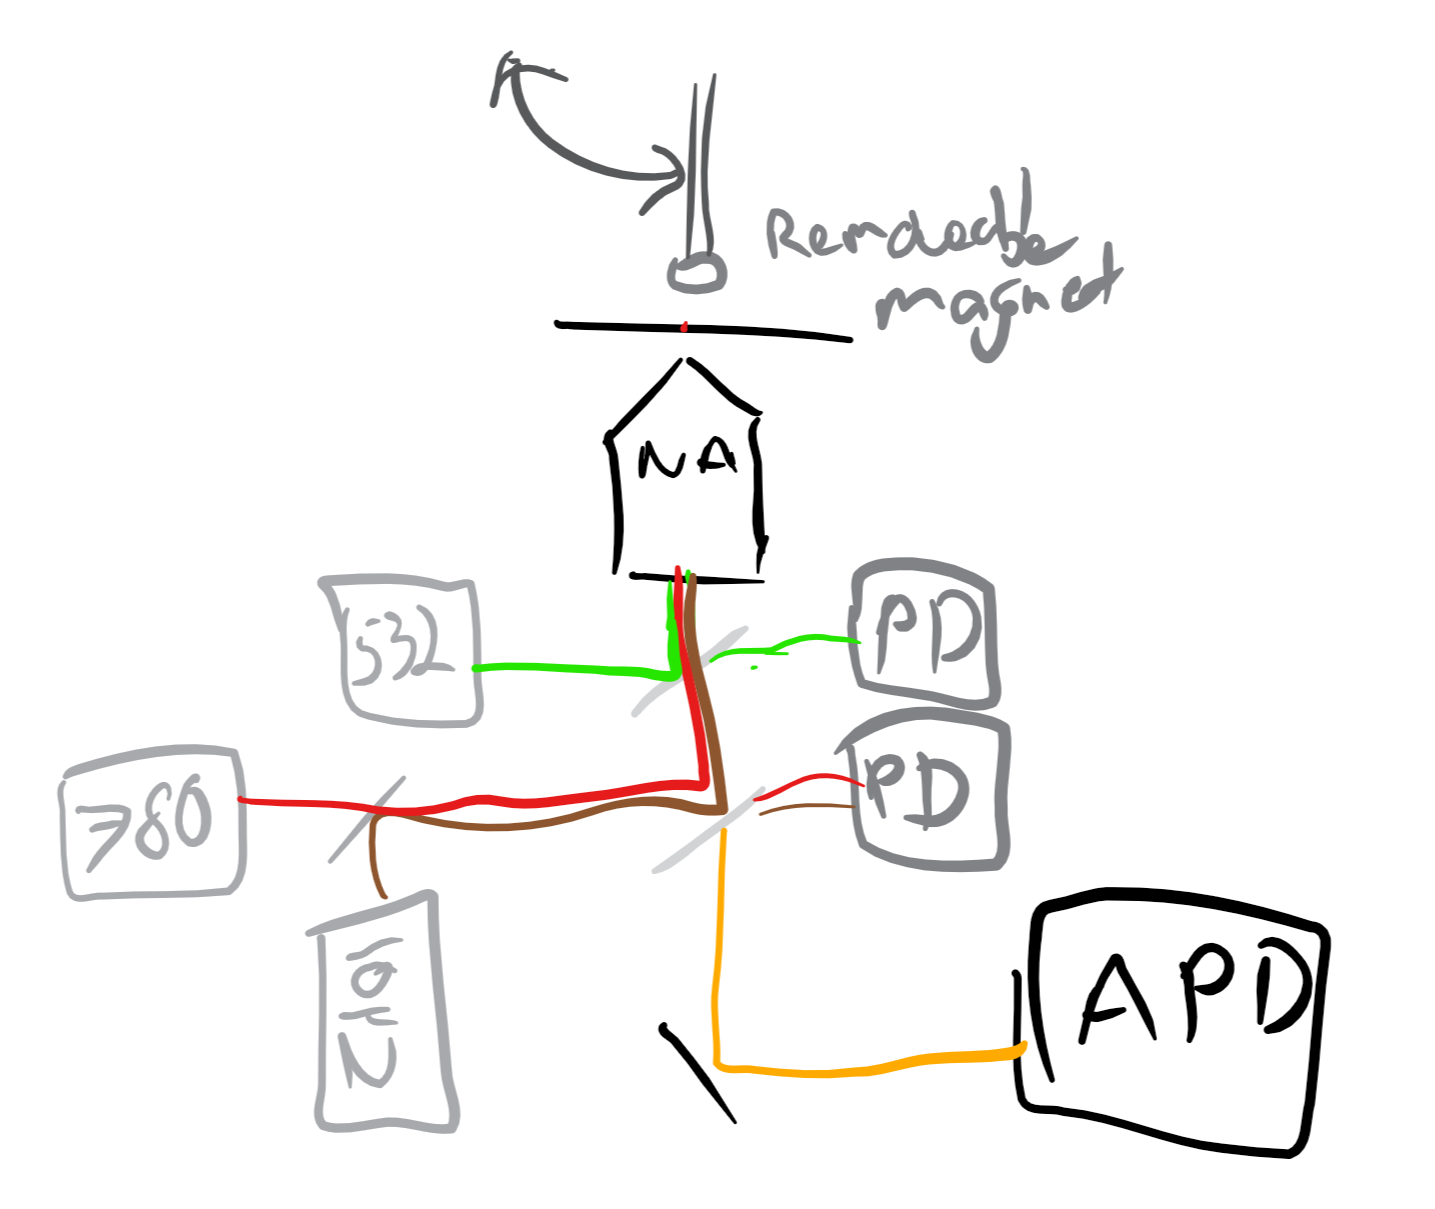
\includegraphics[width=0.5\textwidth]{Setup.png} 
 \caption{\textbf{Experimental approach.} This is the setup ???} \label{FigSetup}
\end{figure}

\subsection{Data Collection}
We start by collecting a saturation curve of the fluorescence of the NV centre. We then investigate the power dependance of the fluorescence on each of the NIR lasers for ??? powers of the green. We place a neodymium magnet \~0.5mm above the sample plane of the confocal microscope in order to mix the spin state of the NV- charge state as described in \S model. Once placed we repeated the above set of measurement. This was repeated for x??? nanodiamonds. The NIR power dependance on the fluorescence of ND??? at ???uW of 532nm is plotted in Fig a. (one with most quenching) and shows that ??mW of NIR laser can suppress fluorescence over ???\%.

\begin{figure}[H]
  \centering
  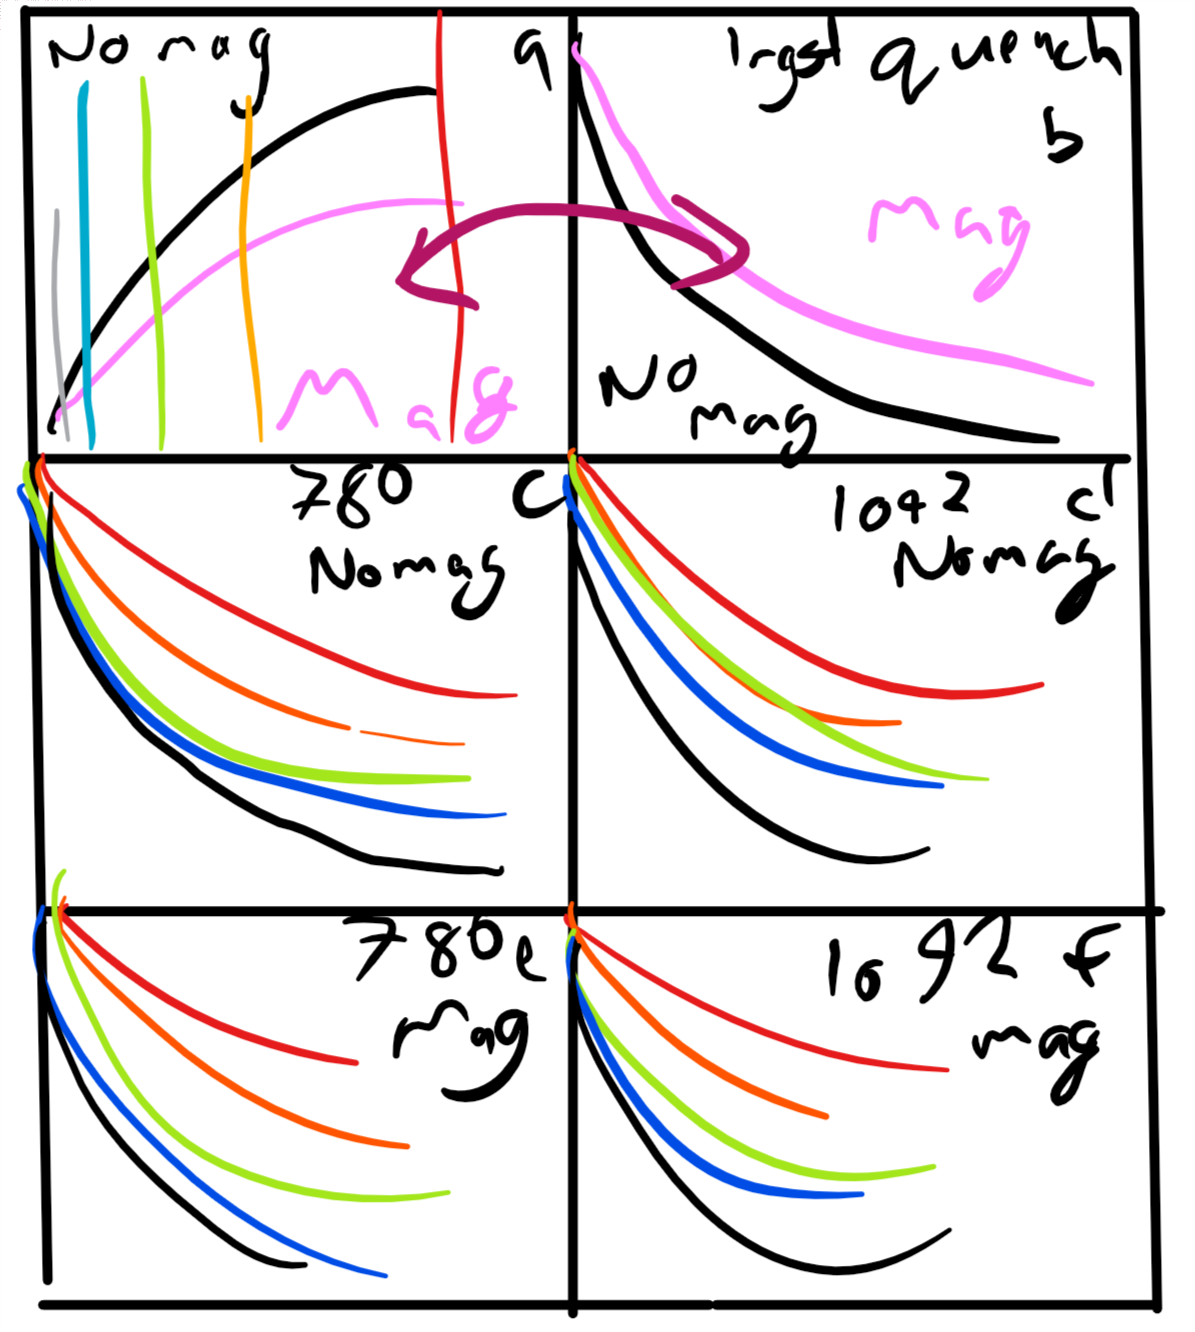
\includegraphics[width=0.5\textwidth]{Data.png} 
 \caption{\textbf{Experimental data.} \textbf{a.} This is the data swap a and b???} \label{FigData}
\end{figure}

\todo{Describe what the data is and what it indicates. Don't bury the lede!}
\todo{I many also want to look at the quenching isolating each window to have an indication if the charge states are quenching equally or not}

\section{NV charge state structure and processes}
\subsection{NV$^-$}
The energy level diagram of the two NV centre charge states and corresponding transition rates can be observed in Fig. \ref{FigEnergyLevels}.

\begin{figure}[H]
  \centering
  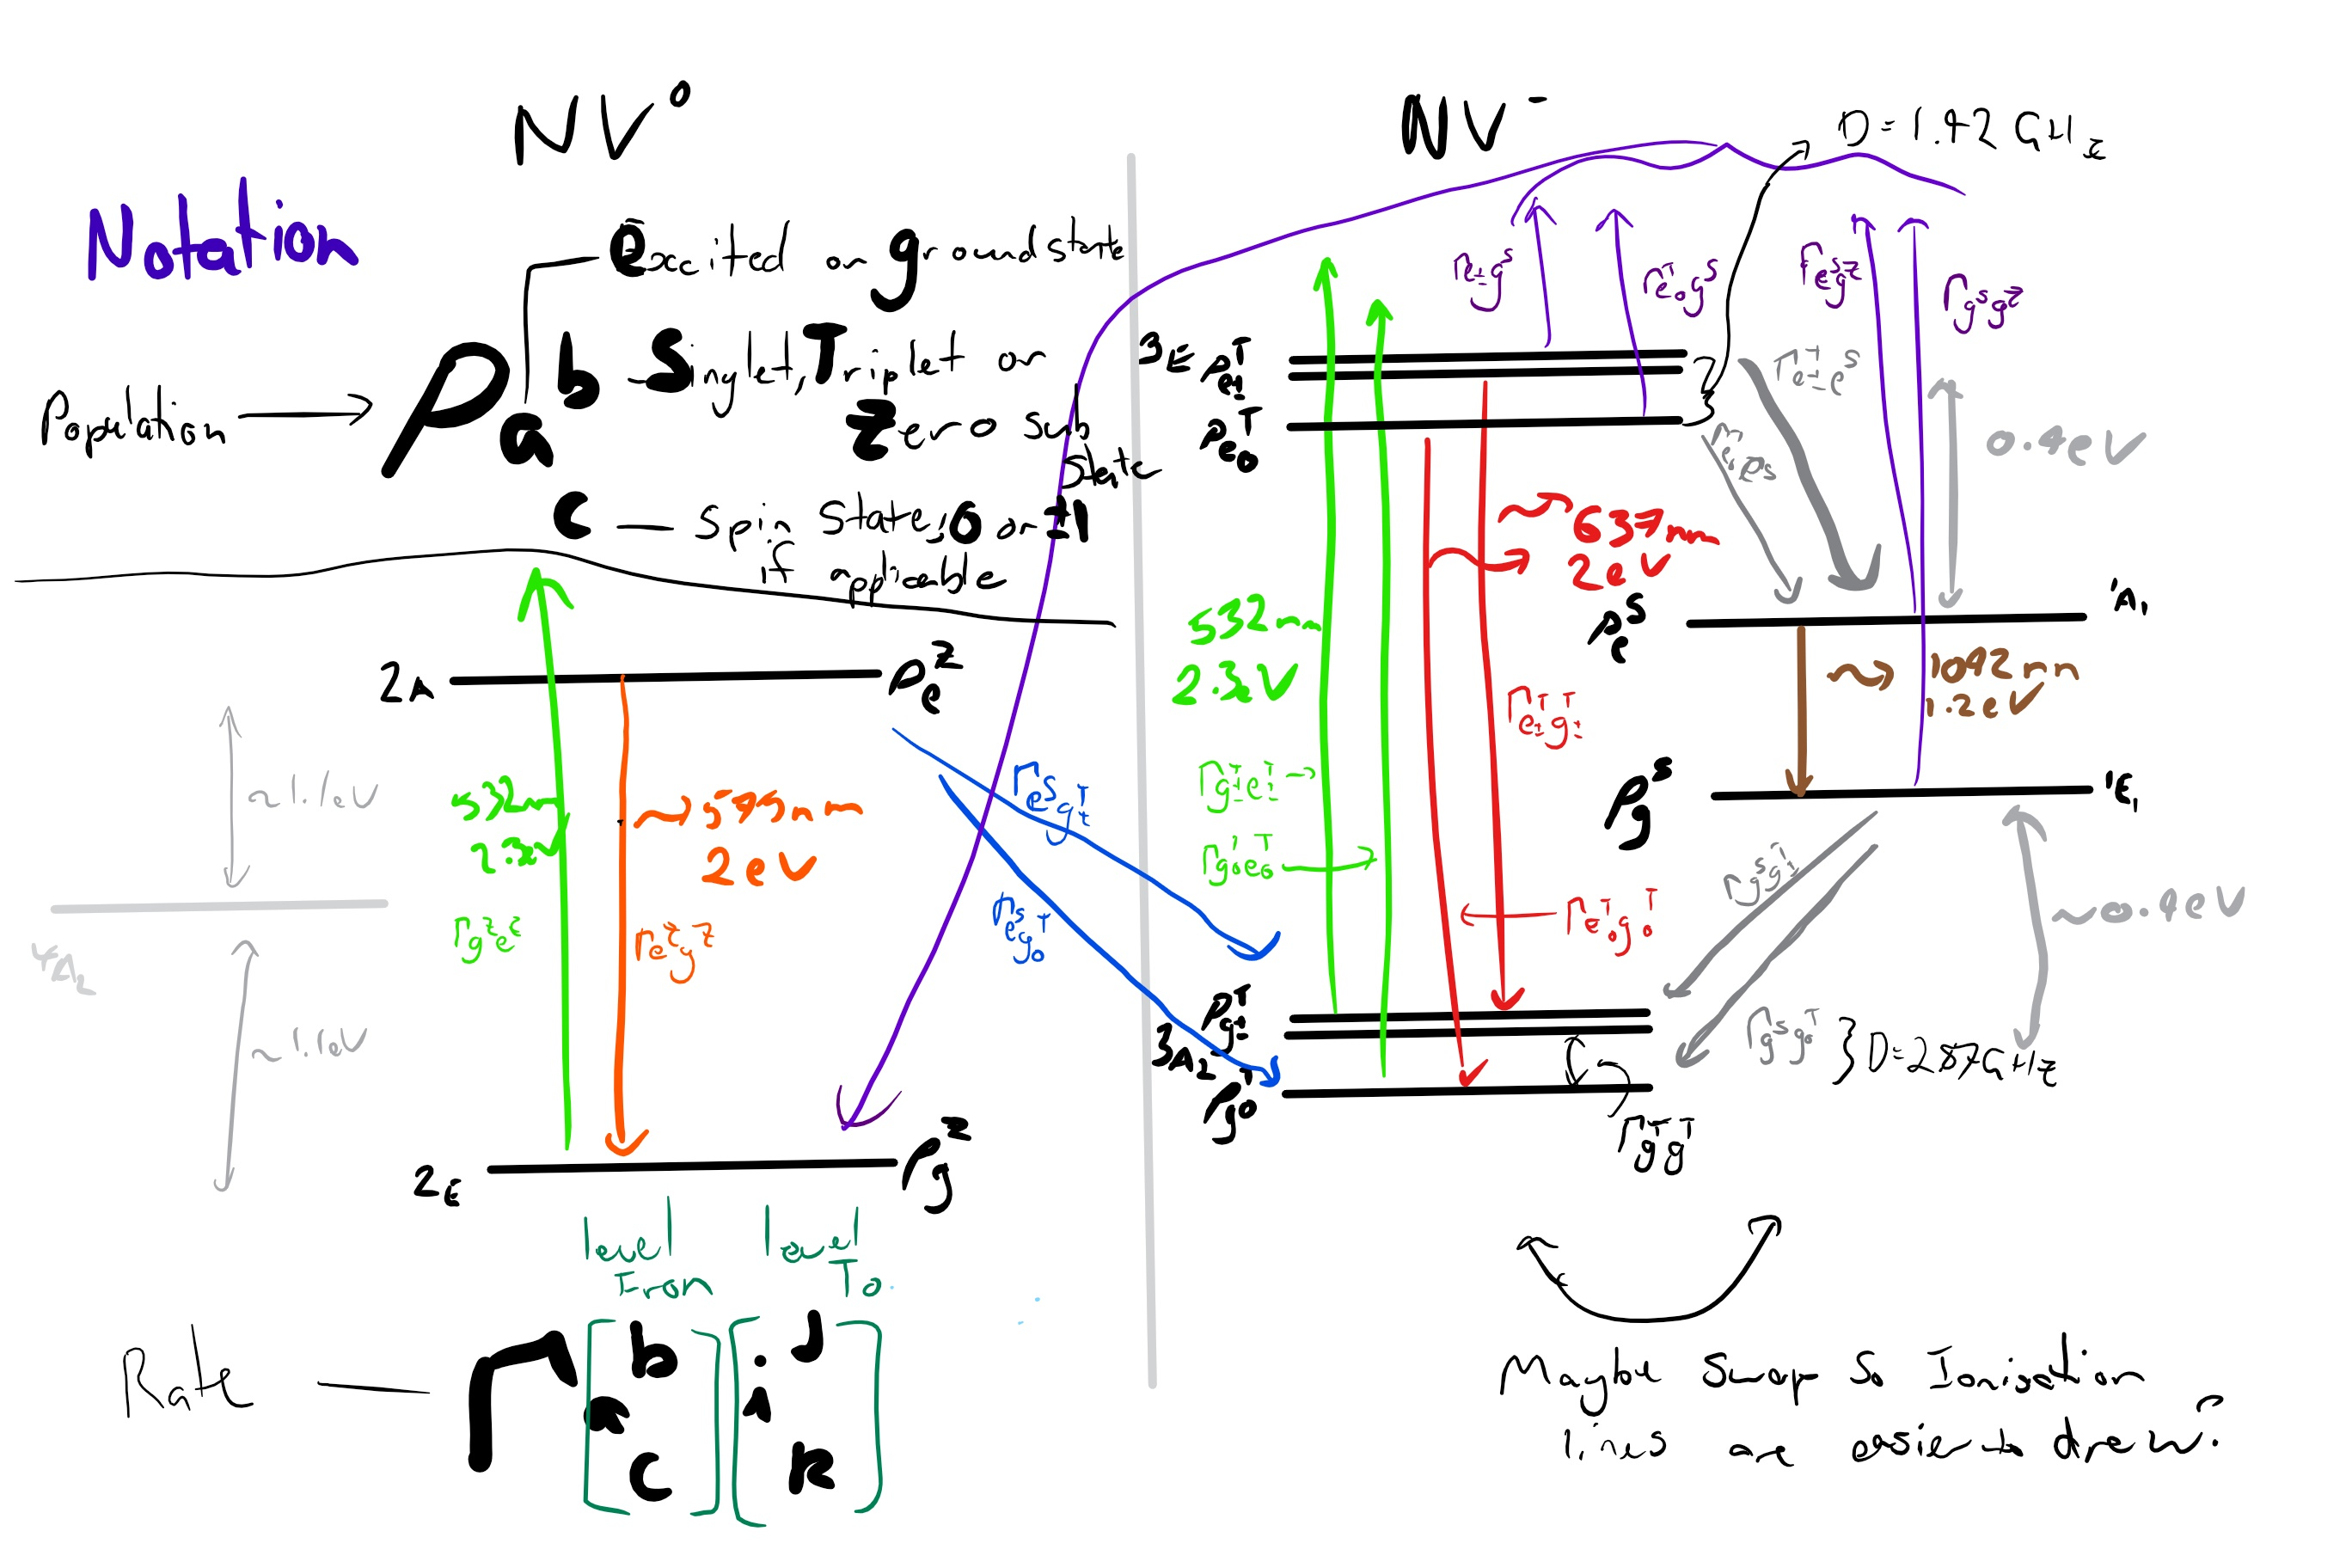
\includegraphics[width=1\textwidth]{NVjpg.jpg} 
 \caption{\textbf{Experimental data.} \textbf{a.} Energy levels rates and notation} \label{FigEnergyLevels}
\end{figure}
\todo{I have include singlet level ionisation in this image but haven't added it to my Matlab code. Don't particularly want to add 2 rates one for each singlet state. If no cycling is observed with 1042nm. I am tempted to compress singlet states into a single energy level since lifetime of excited<<lifetime of ground. Additionally I have not included a STED like mechanism for the NV$^0$ charge state which I probably should do..???}


The photo-physics of the isolated NV- charge state has been well studied and we utilise the established six state model to describe its intrinsic dynamics that includes its internal spin state. It consists a ground triplet state $^3A$ and an excited triplet state $^3E$, as well as two metastable singlet states $^1E_1$ and $^1A_1$ ref11???. The ground and excited triplet states can be further split into three spin levels, $m_s=0$ and $m_s=\pm1$ which are degenerate at zero magnetic field. The energy difference between the spin sublevels $m_s=0$ and $m_s=\pm1$ is $D=\SI{2.87}{GHz}$ for the ground state and $D=\SI{1.42}{GHz}$ for the excited state, where D is the zero field splitting ref12???. The transition rate between $m_s=0$ and $m_s=\pm1$ sublevels is given by the spin-lattice relaxation $T_1$ and has been measured to be $\Gamma_{g^Tg^T} = \sim\SI{6}{ms}$ at room temperature and zero magnetic field ref13???. This spin mixing rate can be increased dramatically by applying a large magnetic field in the vicinity of the NV centre ref14???.
\todo{I am being vague about the spin mixing rate because because I believe the current explanation of Zeeman splitting the spin sublevels has holes in it. Ask me for more info or look at comment in tex file}
% This explanation would not explain the saturation effect that are observed as you bring in the magnet. Following the Zeeman splitting logic you would expect only one spot where there is large mixing and then you would reduce the mixing as you cross this precise field strength. However this saturation effect may be a result of having a collection of NV centres, however Xavi and Matt observed the same effect with single NV centres. This leads to the belief that the spin mixing may not be due to zeeman splitting and the absolute magnitude of the magnetic field but instead due to the thermal perturbations of the magnet destroying the spin coherence. In any case someone familiar with NV centres will accept this statement anyway. Although the question of why there is no spin mixing on the excited state is still a valid question that I still have no answer for other than it is completely absent from the literature and at this stage (22/12/16) my model does indicated that it does not occur. 	I also had the thought that the spin mixing rate is still increasing as we are bringing in the magnet but the rate is already high enough to spin depolarise the system. This can be checked using the model.
%If they were only capturing NV- or mostly NV- (I Never got a good answer to this question from MAtt and Xavi) then due to a combination of the magnet mixing the spin state, which will give an \~\%30 quenching by it self, and then due to spin dependant ionisation this mixed spin state will lead to a higher Ionisation rate and hence a reduction in NV$^-$ charge state polarisation and reduction in Fuorescence.

The main triplet $^3A-^3E$ transition has a Zero Phonon line of 637nm and can be efficiently excited with spin conservation at most wavelengths below 640nm ref15???. We excite this transition at a wavelength of 532nm and the excitation rate increases linearly with incident intensity ($\Gamma_{g^Te^T} \propto I_{532}$). The radiative lifetime of the excited state is 13ns for NV centres in bulk diamond ref16??? and approximately $\Gamma_{e^Tg^T} = \SI{25}{ns}$ for NV centres in nanodiamonds ref17???. Only a few percent of the Fluorescence is emitted at the ZPL, most fluorescence appears in the phonon side bands between 600 and 800nm as shown in Fig. \ref{FigFluoro}.

\begin{figure}[t]
  \centering
  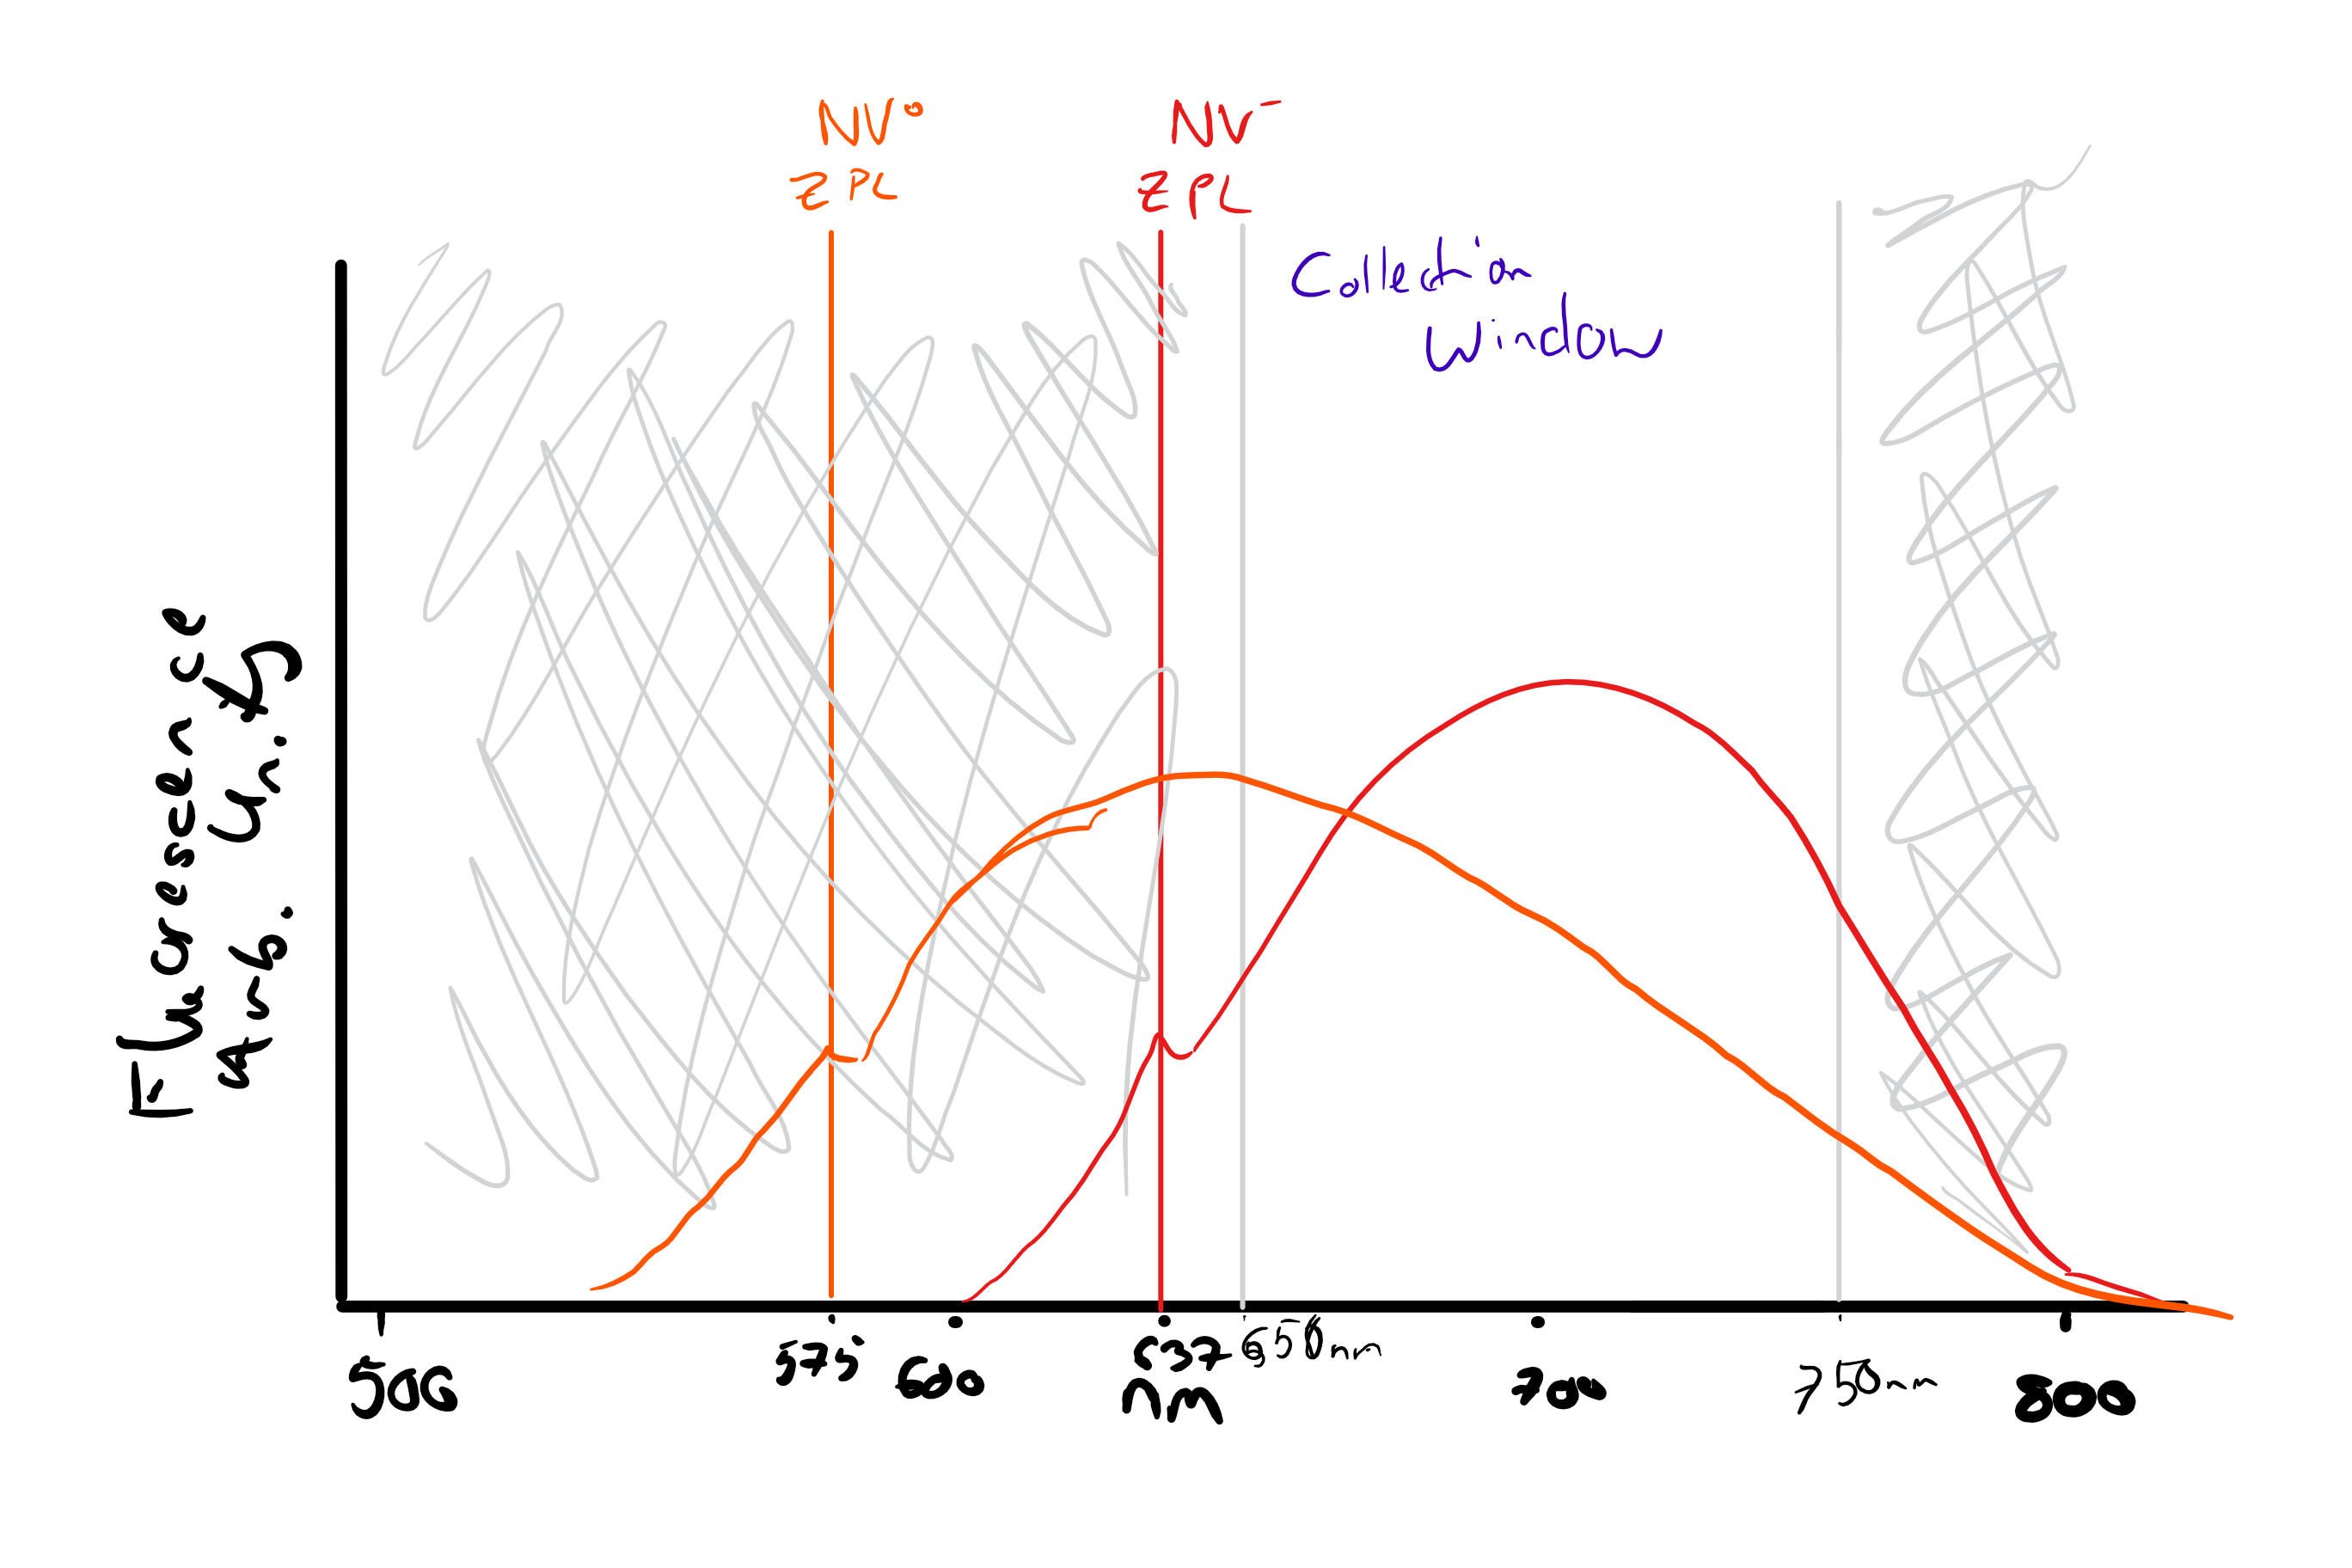
\includegraphics[width=1\textwidth]{Fluoro.png} 
 \caption{\textbf{Experimental data.} Fluoreschece profiles of NV charge states .} \label{FigFluoro}
\end{figure}

The excited triplet states can also decay to the excited singlet state, the rate from the $m_s=\pm1$ excited triplet state is $\Gamma_{e^T_{\pm1}e^S} = 2\pi\times9.4\times10^6\SI{}{GHz} = \SI{16.9}{ns}$, whereas the rate from the $m_s=0$ excited triplet state is almost an order of magnitude smaller at $\Gamma_{e^T_{0}e^S} = 2\pi\times1.8\times10^6 \SI{}{GHz} = \SI{88.4}{ns}$ ref18???. Whilst it not completely understood why there is a large discrepancy between these decay channels it is noteworthy that this discrepancy is what leads to many of the interesting optical properties of the NV centre. It causes a difference in fluorescence intensity between the two excited spin states which in turn leads to a mechanism for an all optical readout of the centres internal spin state. The excited singlet state lifetime is then $\Gamma_{e^Sg^S} = \si{1}{ns}$ ref19??? which has been shown to emit fluorescence at a ZPL of $\SI{1042}{nm}$ ref20???. The longer lived ground metastable state has a lifetime of $\Gamma_{g^Sg^T} = \SI{150}{ns}$ and decays into the ground the triplet spin state ref21???. It was commonly believed that this population decayed only into the $m_s=0$ spin state leading to the spin state polarisation observed in NV centres, however a recently this is being challenged and it has been claimed that the decay into the ground triplet has a spin state ratio closer to $\frac{m_s=0}{m_s=\pm1} = 1.1-2$ ref22???. 

\subsection{NV$0$}

As opposed to the rigorous study the NV$^-$ charge state has received the $NV^0$ charge state has often been neglected. However in order to study the NV centre it must be included. We use the established three level model to describe its intrinsic dynamics. The NV$^0$ consists of a ground doublet $^2E$ and an excited doublet $^2A$ with a ZPL at $\SI{575}{nm} = \SI{2.156}{eV}$  and can be efficiently excited at most wavelengths below $\SI{675}{nm}$ ref23???. Differing from NV$^-$, NV$^0$ does not have detectable magnetic resonances associated with its spin doublet ground and excited states ref24???. We excite this transition with the same 532nm laser as used for the NV$^-$ and the excitation rate increases linearly with incident intensity ($\Gamma_{g^Ze^Z} \propto I_{532}$). Although the exact excitation cross section is unknown the ratio of excitation cross sections between NV$^0$ and NV$^-$ can be measured by looking at their relative emission intensities. The ratio of excitation cross sections is $\Gamma_{g^Ze^Z} = \frac{1}{3} \Gamma_{g^Te^T}$ ref25???. The radiative lifetime of the excited state is $\Gamma_{e^Zg^Z} = 19\times2 \SI{}{ns}$ ref26???.  
\todo{I think I doubled this value because NV- lifetimes were doubled in ND as compared to bulk and the lifetime I found was in Bulk diamond. Either need to find value for ND's or argue that it should also increase the same way as NV- did...} Only a few percent of the Fluorescence is emitted in the ZPL, whereas most fluorescence appears in the phonon side bands between 550 and 800nm as shown in Fig \ref{FigFluoro}. The third energy level attributed to the NV$^0$ is a metastable spin quartet $^4A_2$ which was measured though an electronic parametric signal ref27. However, no ODMR or optical readout of this metastable quartet have been measured and it is expected to have negligible impact on the photo-physics of the NV centre and as such has been neglected from our analysis. \todo{This statement was true as of February 2013, I need to ensure that this is still true.}

\subsection{Charge State Conversion}
To convert between the two charge states we need to examine both the Ionisation process from NV$^-$ to NV$^0$ and  the Recombination process from NV$^0$ to NV$^-$.

\subsubsection{Ionisation}
Ionisation from NV- to NV0 occurs in a two step process as shown in Fig. \ref{FigChargeConversion}.

\begin{figure}[H]
  \centering
  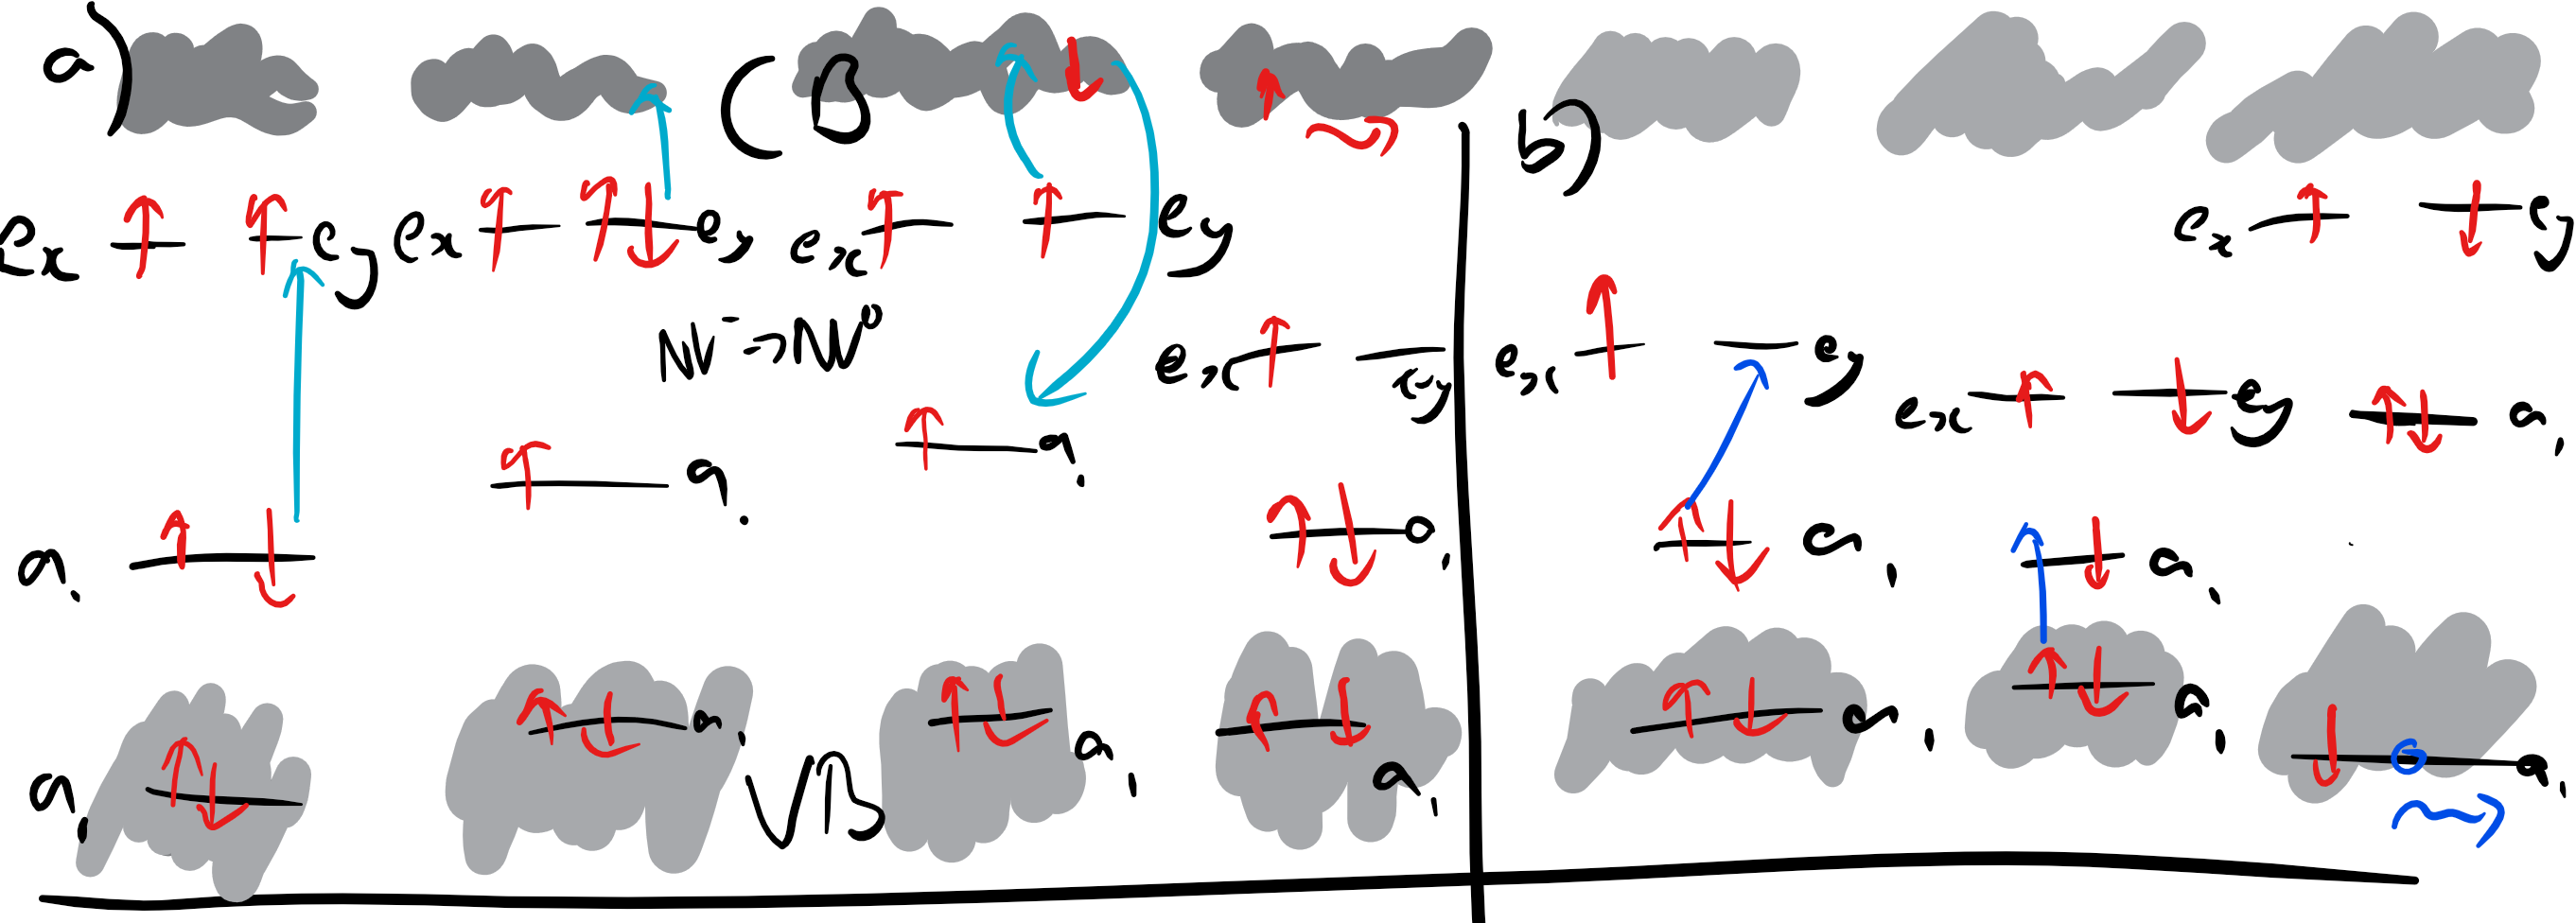
\includegraphics[width=1\textwidth]{ChargeConversion.png} 
 \caption{\textbf{Charge State Conversion Processes.} \textbf{a,} Ionisation from NV$^-$ to NV$^0$ \textbf{b,} Recombination process from NV$^0$ to NV$^-$ figure of ionisation and recombination processes with the quadratic dependence} \label{FigChargeConversion}
\end{figure}

First a photon must must excite an electron into the excited $^3E$ state of the NV$^-$ and then another photon must promote an excited electron into the conduction band leading to an Auger Ionisation process which strips an electron off of the NV$^-$ centre and converts it into the NV$^0$ in its ground state configuration ref28???. The electron of the NV$^-$ can also be promoted from singlet metastable states to the conduction band leading to an auger ionisation process if the photon energy is higher than the corresponding energy barrier.

\subsection{Recombination}
The recombination process from NV$^0$ to NV$^-$ also occurs in a two step process which is shown in Fig. \ref{FigChargeConversion}b. First a photon must excite the NV$^0$ charge state, and then a second photon can promote an electron from the valence band into the $^2E$ ground state providing an extra electron to the centre converting it into the NV$^-$ in its ground state configuration ref29???. Currently there is no evidence to indicate which spin state the NV$^-$ charge state will now be populated in, however it has recently been observed that the ionisation, recombination process is a spin depolarising process indicating a non negligible component in the $m_s=\pm1$ spin state ref30???. The result of both the ionisation and recombination process is that with a single excitation wavelength the charge state conversion rates increase quadratically with excitation intensity. The process has been studied for a variety of excitation energies in order to determine the optimal excitation wavelength in order to provide the largest NV$^-$ charge state polarisation ref31???, however this analysis only investigated from $\SI{450}-\SI{610}{nm}$ with a single wavelength at any one time. As a result many people in the NV community will excite the defect with a wavelength from $\SI{510}{nm}-\SI{540}{nm}$, typically $\SI{532}{nm}$.

Howevera, as a result of exciting both the NV$^0$ and NV$^-$ with the same wavelength the recombination process has only been observed with wavelengths less than or close to the ZPL of the NV$^0$ at $\SI{575}{nm}$. We believe however that one can excite the transition with a wavelength $<\SI{575}{nm}$ satisfying the first stage of the recombination process and then promote electrons from the valance band with a wavelength longer than $\SI{575}{nm}$. It has been proposed also that the conversion from NV$^0$ to NV$^-$ is mediated by ionisation of single substitutional Nitrogen impurities ($N_s$) in the nanodiamonds providing free electrons to combine with the NV$^0$ charge state ref32???. Ionisation of $N_s$ impurities requires $>\SI{1.7}{eV}$ for bulk diamond and slightly lower energy $>\SI{1.6}{eV}$ for nanodiamonds ref33???. Our nanodiamonds are a highly irradiated sample and therefore contain a high concentration of single substitutional nitrogen $N_s$. We postulate that the quenching observed in our nanodiamonds could be due to an dramatic increase in the ionisation and recombination rates induced by the NIR lasers and developed a rate equation model to determine the likelihood of this process compared to a STED like mechanism.

\subsection{Model}
In order to determine the intrinsic photophysics of our nanodiamonds we developed an 8 level rate equation model that incorporates both the ionisation and recombination mechanisms as well as the STED like mechanisms. It is important to note that whether the STED like effect is simply non radiative decay from the excited to ground triplet state ref34??? or is mediated through a new fast decaying dark band ref35??? the mechanisms reduce to identical rate equations. The population of each NV energy level can be described by determining the valid transition rates between each energy level as shown in Fig. \ref{FigEnergyLevels} which are given by;
\begin{eqnarray}
\dot{\rho_{e^{T}_\pm}} & = & blah\\ 
\dot{\rho_{e^{T}_0}} & = & blah\\
\dot{\rho_{g^{T}_\pm}} & = & blah\\ 
\dot{\rho_{g^{T}_0}} & = & blah\\
\dot{\rho_{e^S}} & = & blah\\ 
\dot{\rho_{g^S}} & = & blah\\ 
\dot{\rho_{e^Z}} & = & blah\\ 
\dot{\rho_{g^Z}} & = & blah.
\label{EqnArray}
\end{eqnarray}

The populations of the energy levels can be solved under steady state conditions and the fluorescence intensity is given by,
\begin{equation}
\SI{}{F} = \left(\rho_{e^{T}_\pm}\times\Gamma_{e^T_{\pm}g^T_{\pm}} +\rho_{e^{T}_0}\times\Gamma_{e^T_{\pm}g^T_{\pm}}\right)+\left(\rho_{e^Z}\times\Gamma_{e^Zg^Z}\right)\times\SI{}{\sigma},
\label{EqnFluoro}
\end{equation}
where F is the fluorescence intensity and $\sigma$ is the ratio between the efficiency of collecting a NV$^-$ photon compared to an NV$^0$ photon, which depends on the fluorescence spectra and the collection window which are shown in Fig. \ref{FigFluoro} as well as the spectral response of the detector. This was calculated to be ??? for our ??? APD with a fluorescence window between $\SI{550}{nm}$ and $\SI{750}{nm}$. For the saturation curves this value can be compared directly against the data with a single scaling parameter $C$, which is related to the effective number of NV centres and collection efficiency, whereas for the NIR quenching data the data can be compared directly by normalising to the fluorescence intensity with no NIR laser power,
\begin{equation}
\SI{}{Fluorescence\ Counts\ (norm}.) = \frac{F(I_{NIR})}{F(0)}.
\label{EqnFluoroCounts}
\end{equation}

\section{Unknown Questions and Assumptions }
In developing the rate equation model there are three unanswered questions that will affect the photo-physics of the system that need to be investigated. For each question a variety of conjectures were developed in order to generate an array of sub-models. The group of sub-models are obtained by generating the complete set of permutations of the given conjectures. The models are then compared with each other using the Akaike Information Criteria, which provides a measure of the comparative likelihood of a model to fit the given data.

The first question is to determine whether the STED like quenching mechanism itself can explain all of the photo-dynamics of the system or if it necessary to include the ionisation, recombination mechanism. Four permutations are investigated to fit the data; Using only a STED like mechanism which will inevitably ignore the NV$^0$ charge state, using a STED like mechanism as well as an ionisation and recombination process mediated only by the $\SI{532}{nm}$ excitation laser, using the STED like mechanism and the ionisation and recombination process mediated by both the $\SI{532}{nm}$ excitation laser and the NIR laser and lastly by leaving out the STED like process and using only the ionisation and recombination process mediated by both the $\SI{532}{nm}$ excitation laser and the NIR laser.
Secondly, it is unclear how the electrons recombine into the into the NV$^-$ ground state from both the metastable state and from the NV$^0$ charge state, the traditional notion and our first conjecture is that the singlet rate decays only into the $m_s=0$ spin state and that the there is no favourable transition for the recombination process, for generality we also provide a case in which there is no limitation on either combination ratio. \todo{Optional:We are however assuming in both of these cases that the presence of a strong magnet field does not effect the energy level favourability of the ground triplet state and hence provide another case where the recombination ratios may change with the presence of the magnet. (I cam up with this effect to explain the \%50 quenching observed by Xavi and Matt due to only the magnet but I beleive that can now be explained without this mechanism. If you want some details about why I think you can actually get \%50 due to the magnet just ask me} Lastly, no investigation has been made into the spin dependency of the ionisation process. These energy levels already exhibit spin dependant rates to the metastable singlet state, and additionally there is a permanent dipole that is an order of magnitude larger for the $m_s = \pm1$ excited spin state than there is for the $m_s=0$ spin state which we believe has the potential to lead to a spin dependant ionisation process ref36???. As a result we do not want to limit our potential models to having only a spin independent ionisation process and hence provide two more cases; a completely spin independent case and a case where spin independent process has the same ratio for both the $\SI{532}{nm}$ and NIR laser. The sub-models were generated from these assumptions and fitted to the data. A summary of all of the various conjectures and sub-models as well as fitted parameters can be found in Tab. or Fig.

\begin{figure}[H]
  \centering
  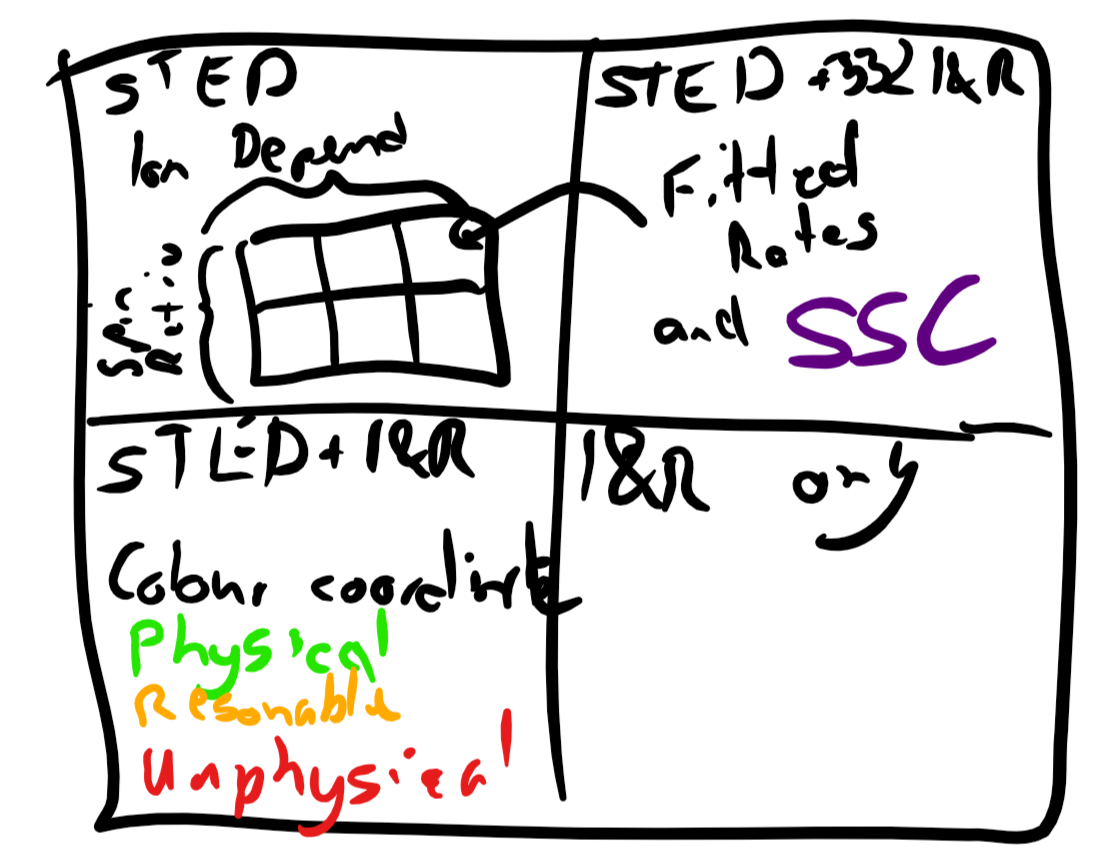
\includegraphics[width=0.4\textwidth]{SubModels.png} 
 \caption{\textbf{Overview of assumptions.} Need to determine a good way of presenting this information.} \label{FigSubModels}
\end{figure}

\todo{If I use the 1042nm laser I also have to include cycling of the transition}

\todo{The rest of the sections that the paper requires or will be much easier once the whole set of data is collected.}



\section{Akaike Information Criteria}
From the minimisation value we can perform an Akaike.
Blah blah statistical analysis of models and assumptions.
top model is blah, investigate it.

\section{Discussion}
Really look into the model that the Aikike has pointed out

\section{Compare Models}
For instance if all models give a similar answer to one variable we can be more confident of this value. Additionally if the models with STED give zero rates for STED the aikike will point out that the model without STED will be more likely. This is due to the fact that the STED rate has a small and mostly negligible effect and that both models are actually converging to the same physics.

\section{Spin Dependant Ionisation}
Explain the spin dependancy and anything else interesting the model picks up that may be unusual. ie look at the validity of the assumptions it used.


\section{Compare the spin state and charge state}
The spin and charge state is interesting because it is completely unconstrained and give a pretty accurate answer.
\section{Give other examples of how this model fits with data}
There are some physics papers with weird mechanisms that this model can explains. Should I write and give plots to compare?


\section{Prospects for future work and impact}
STED like imaging
How to improve charge state and spin state polarisation useful for quantum applications.

\todo{Maybe think of a nice short name for ionisation and recombination process because I use it so much. Could simply use ionisation and recombination = (I\&R)?}

\section{}



%~\cite{Blancquaert2013} 

%\begin{figure}[t]
%  \centering
%  \includegraphics{figure_2D_setup.eps} 
%  \caption{\textbf{Experimental approach.} \textbf{a,} figa\textbf{b,} figb} \label{FigSetup}
%\end{figure}

%Fig.~\ref{FigAperture}.
%
%\todo{If I can find the original data, I want to treat the "old" data with the new code. In any case, I want to redo the plot with the same colorscale as Fig2.}


\section*{Acknowledgements}

....
%%%%%%%%%%%%%%%%%%%%%%%%%%%%%%%%%%%%%%%%%
%%%%%%%%%%%%%%%%%%%%%%%%%%%%%%%%%%%%%%%%%
%%%%%                                                                                                   %%%%%
%%%%%                                       APPENDIX                                          %%%%%
%%%%%                                                                                                   %%%%%
%%%%%%%%%%%%%%%%%%%%%%%%%%%%%%%%%%%%%%%%%
%%%%%%%%%%%%%%%%%%%%%%%%%%%%%%%%%%%%%%%%%

%
%\appendix
%
%\section{Experimental parameters}
%\label{param}
%




\begin{thebibliography}{27}






\end{thebibliography}




\end{document}
